\section{The Standard Model} \label{sec:SM}

The standard model (SM) is a quantum field theory which defines a set of quantum fields, whose excitations correspond to observable particles, and describes how they interact. The SM is considered one of the most successful and widely encompassing physical theories to date, as it is consistent with most of the phenomena observed in particle and nuclear physics experiment, and therefore forms a bedrock of understanding of the nature of the universe. The SM defines a quantum field for each type of particle, where the particles include force mediating gauge bosons, a scalar boson, and fermions making up massive material. 

The difference between these two classes of particles is as follows: Bosons obey Bose-Einstein statistics, meaning many of them in a given system can simultaneously exist in the same quantum state, while fermions obey Fermi-Dirac statistics, under which no two fermions within a system can exist in the same quantum state. The particles described by the standard model are depicted in Fig \ref{fig:SM_Diagram}.  

%%-- Standard model diagram 
\begin{figure}[H]
    \centering
    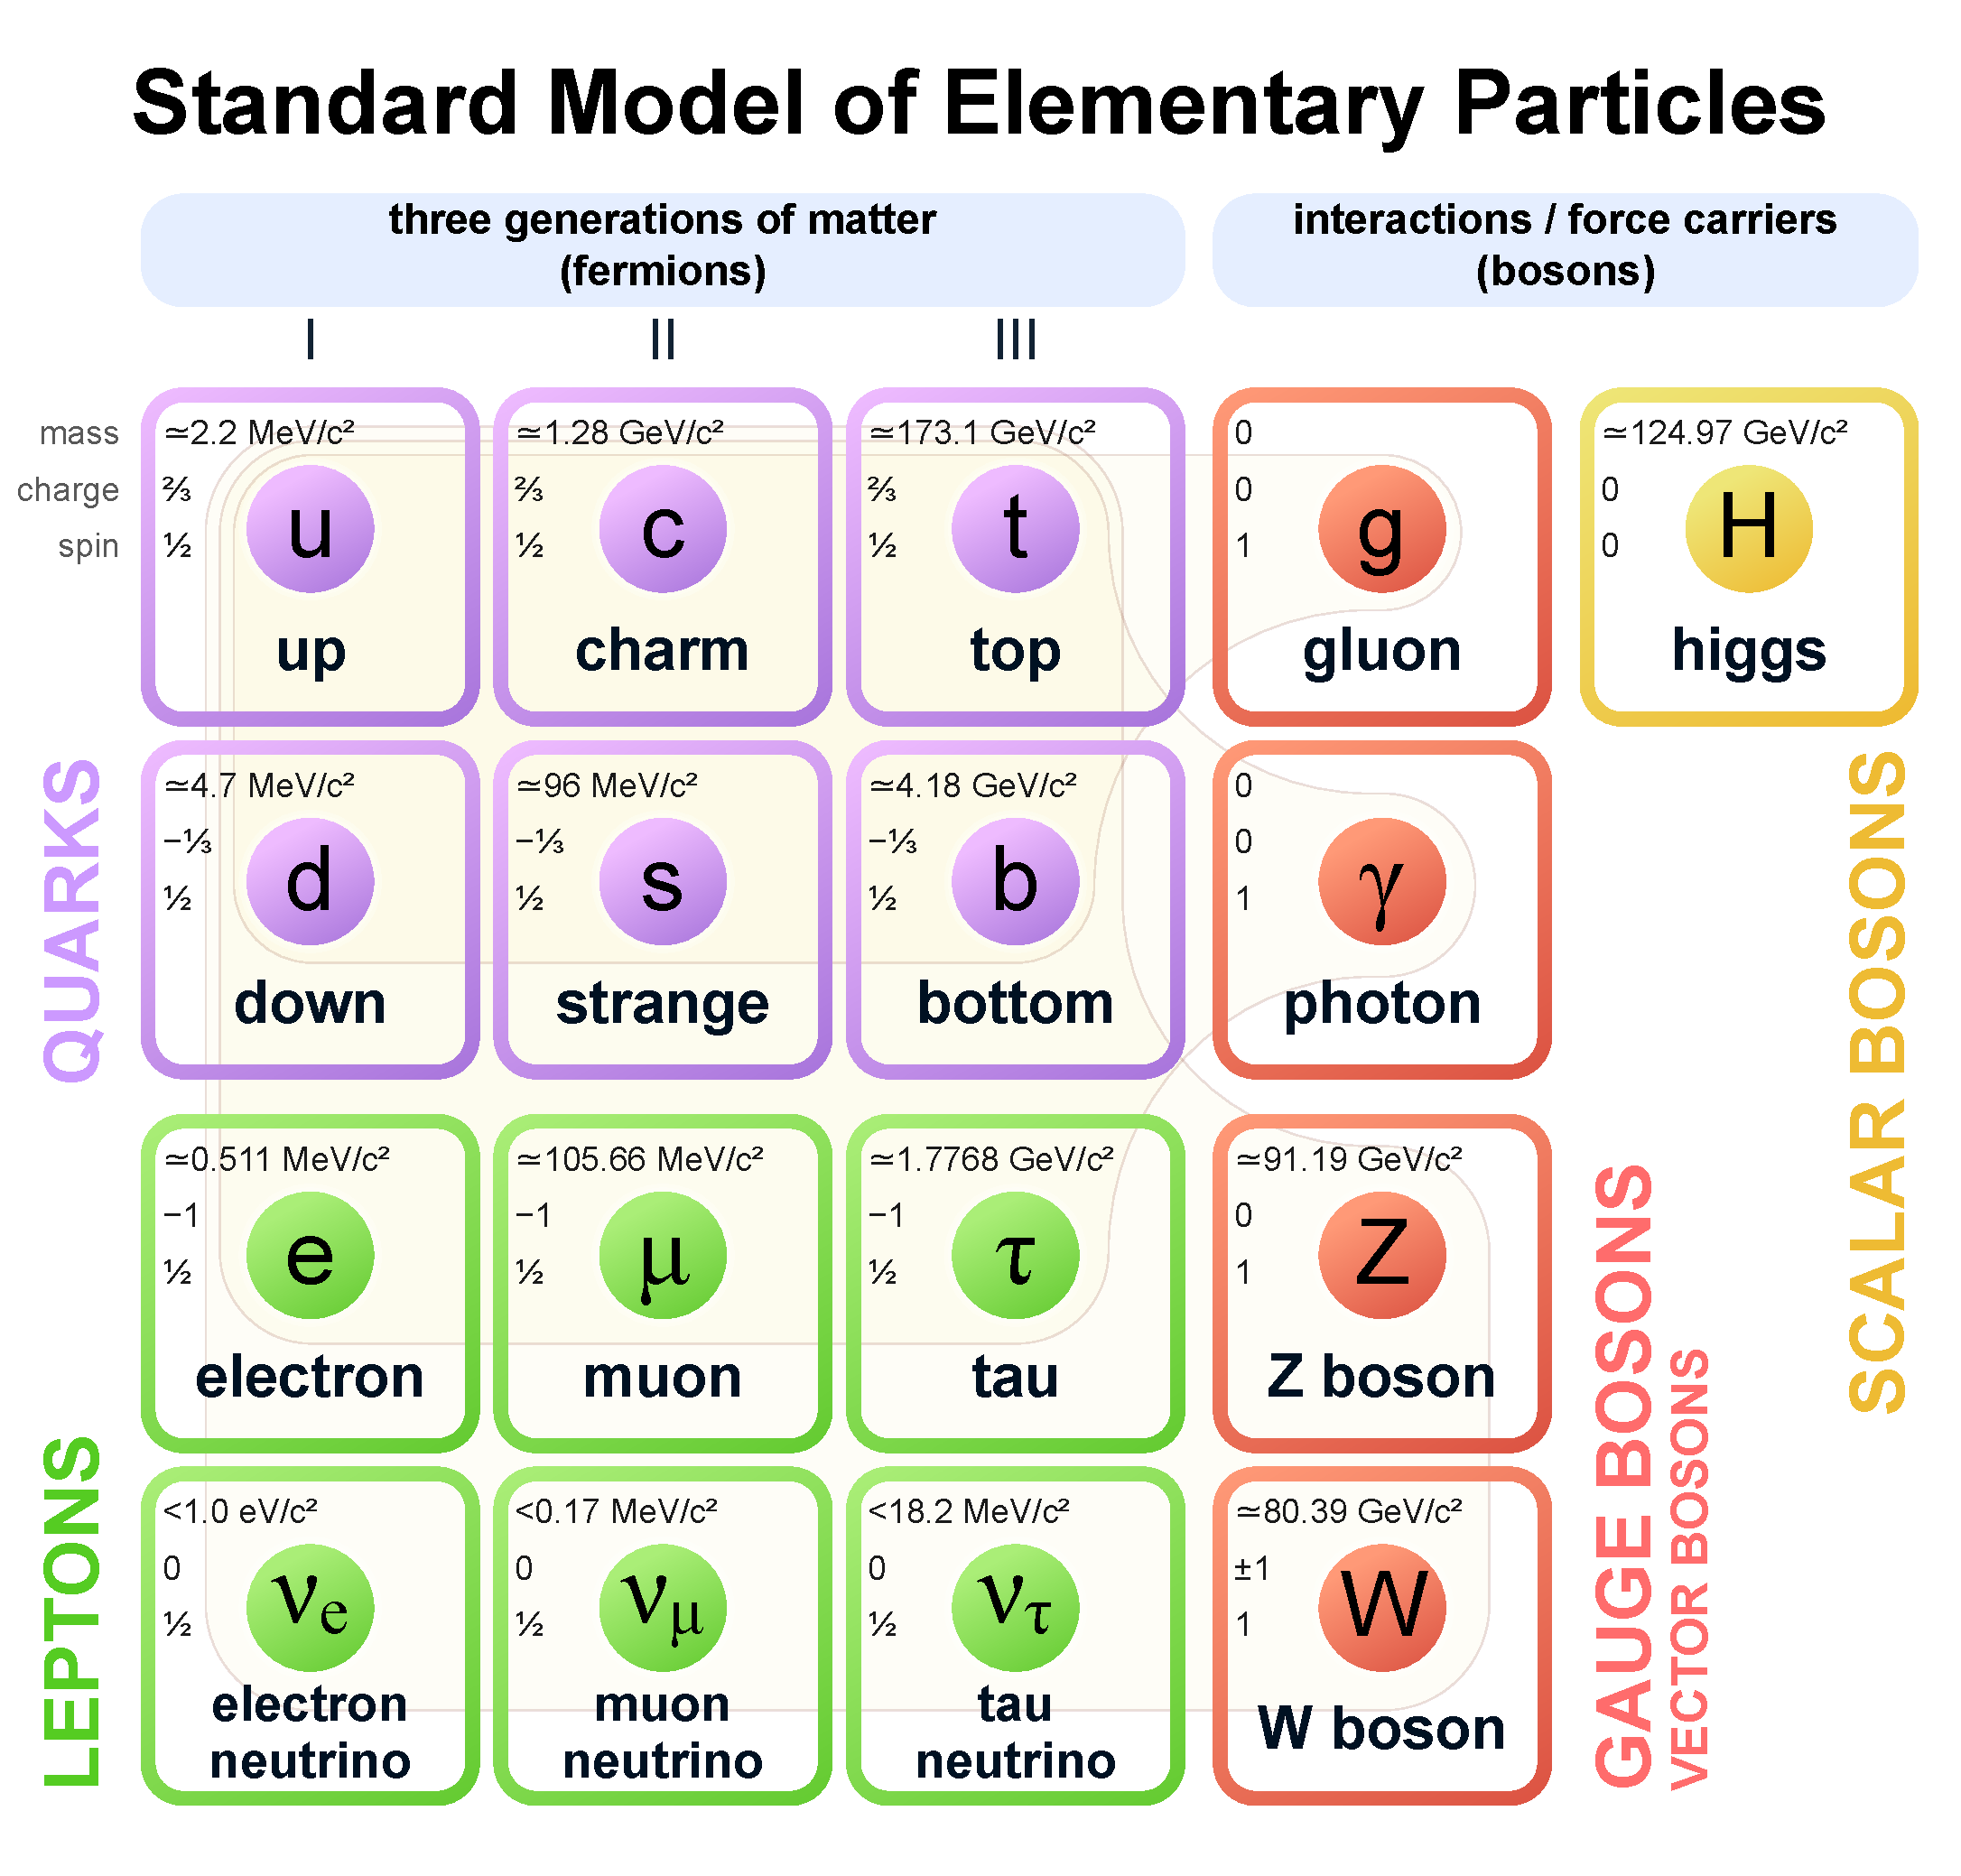
\includegraphics[width=\textwidth]{Images/Theory/Standard_Model_of_Elementary_Particles.pdf}
    \caption{Particles described by the Standard Model}
    \label{fig:SM_Diagram}
\end{figure}

An important feature of the SM lagrangian is its invariance under the product group shown in Equation \ref{eq:ProductGroup}.

\begin{equation} \label{eq:ProductGroup}
    SU(3)_{C}\times SU(2)_{W}\times U(1)_{Y}
\end{equation}

The invariance of the SM lagrangian under these gauge groups corresponds to the conservation of color charge, weak isospin, and hypercharge. In addition, these gauge groups correspond to three fundamental forces: The electromagnetic force mediated by the photon (U(1)), the weak force mediated by the $W^{\pm}$ and Z bosons (SU(2)), and the strong force mediated by the gluon (SU(3)). A known fourth fundamental force of nature, the gravitational force, is not described by the standard model. The absence of the gravitational force in the standard model is a sign that while the SM explains the majority of observations, it is an incomplete description of the fundamental particles and interactions of the universe. 

\subsection{Particles}

The SM predicts the existence of particles, which manifest in observation as excitations of their corresponding quantum fields. The particles are classified as fermions described in Section \ref{sec:fermions}, and bosons described in Section \ref{sec:bosons}.

\subsubsection{Fermions} \label{sec:fermions}

Fermions are defined as particles which obey Fermi-Dirac statistics, meaning that no two fermions in a quantum system can occupy the same quantum state. At a macroscopic scale, this can be qualitatively thought of as the impossibility for two pieces of matter to go through each other. At a microscopic scale, one implication of Fermi-Dirac statistics is that as an atom gains more electrons, they must occupy ``shells'' at higher energy states, as lower energy states may already be occupied by existing electrons. 

The two types of fermions are quarks and leptons, each of which has three generations, increasing in mass with each generation. The quarks are composed of up and down (1st generation), charm and strange (2nd generation), and top and bottom quarks (3rd generation). When describing particle masses, the base unit used is the electronvolt (eV), where 1 eV corresponds to the amount of kinetic energy gained by an electron when accelerated from rest across one volt of electric potential in a vacuum. The six SM quarks have a large mass range spanning a few MeV up to 173 GeV (current mass measurement of the top quark), and account for the quantum numbers of hadrons. A common instance of quarks is the composition of the most common hadrons we see around us: Protons (neutrons) have three valence quarks: two up (down) quarks and one down (up) quark.

% https://en.wikipedia.org/wiki/Color_confinement

In the SM, quarks are predicted to be confined, meaning they cannot exist freely and must always be in a bound state with other particles. This means when quarks are produced in experiment, such as from particle collisions, these quarks immediately form pairs with quarks from the QCD vacuum. This process continues with subsequent quarks, leading to the detection of a jet of hadronic activity rather than a single quark. This phenomenon is called hadronization, and is shown in Figure \ref{fig:Quark_Hadronization}. This phenomenon is constantly seen at hadron colliders, and is a fundamental handle for detecting quarks and gluons.

\begin{figure}[H]
    \centering
    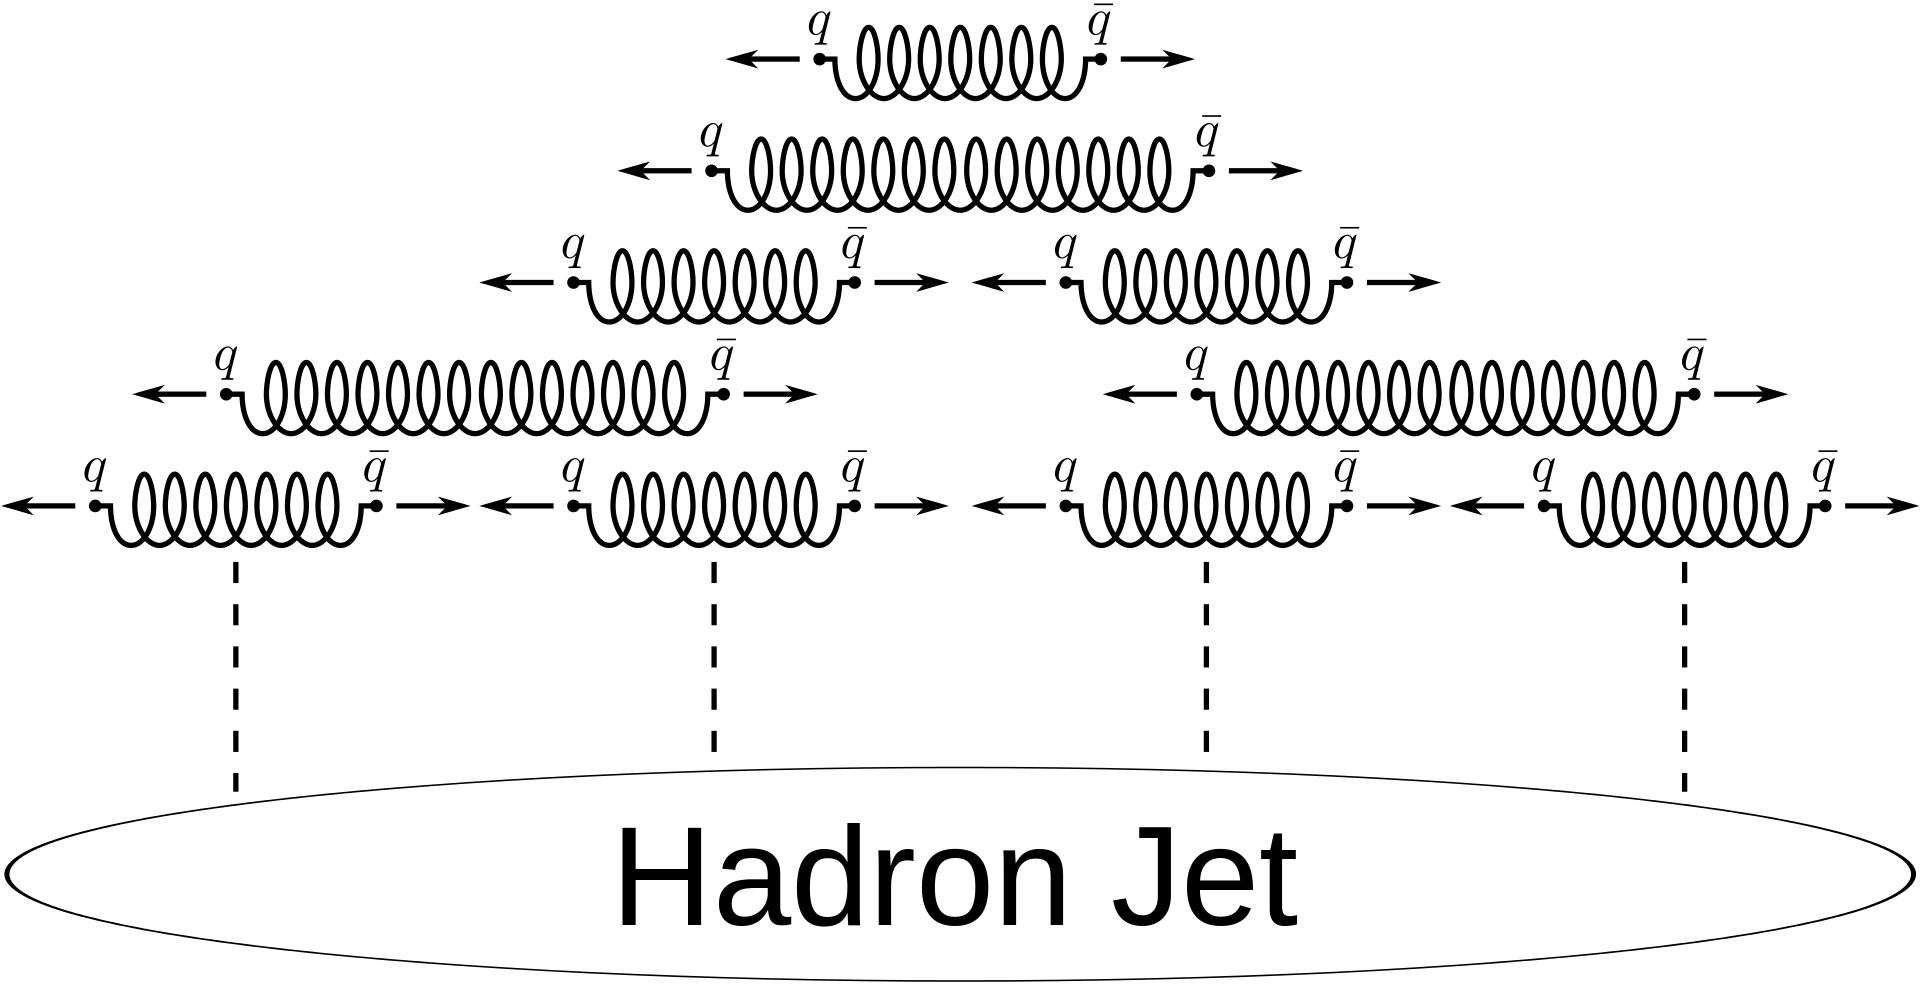
\includegraphics[width=\textwidth]{Images/Theory/Quark_confinement.png}
    \caption{Diagram of quark hadronization}
    \label{fig:Quark_Hadronization}
\end{figure}

The three generations of leptons are the electron, muon, and tau, each with a corresponding flavour of neutrino. Electrons are present in atoms, as they exist in quantum states surrounding the atomic nucleus comprised of neutrons and protons. 

While electrons, muons, and taus have mass, in the SM there is no mechanism by which neutrinos gain mass. However, experimental measurements of neutrino oscillations have observed non-zero differences between the squared masses of different neutrino flavors, implying that neutrinos have mass. This is further evidence that the SM is incomplete.  

All leptons also have an associated anti particle, which posses the same traits as its corresponding particle but with a negated electric charge. 

\subsubsection{Bosons} \label{sec:bosons}

Bosons are defined as particles which obey Bose-Einstein statistics. The SM predicts five bosons, namely the gluon, photon, Z boson, W boson and Higgs boson. 

Gluons are responsible for mediating the strong force, the mechanism which keeps protons in a bound state by binding their valence and sea quarks. The energy stored in this binding of quarks via gluons accounts for most of the mass of the proton. 

The photon is a massless boson which mediates the electromagnetic force between charged particles. It is also the particle corresponding what we see as light: Electromagnetic radiation, which at certain frequencies is visible to the human eye. 

% https://cds.cern.ch/record/2103277/files/9789814644150_0006.pdf?subformat=pdfa&version=1

The W and Z bosons mediate the weak force, and were experimentally discovered by the UA1 and UA2 experiments at CERN in 1983.

The quantum field corresponding to the Higgs boson plays the special role of providing the mechanism by which massive fermions and bosons obtain their mass. 

\subsection{Forces}

While predicting the existence of fermions and bosons, the SM also predicts three types of interactions between these particles: The strong, weak, and electromagnetic interactions. 

\subsubsection{The strong interaction}

The strong force is mediated by the gluon, and is the force by which gluons and quarks interact. This type of interaction is called Quantum Chromodynamics (QCD), and corresponds to the SU(3) gauge symmetry in the SM, for which color charge is the conserved quantity. 

This force is crucial to our qualitative conception of matter, as it is responsible for the binding of quarks into protons and neutrons, as well as the binding of protons and neutrons into stable molecules. 

\subsubsection{The weak interaction}

The weak force is a fundamental force mediated by the W$^{\pm}$ and Z bosons, and corresponds to the SU(2) gauge symmetry of the SM, whose conserved quantity is weak isospin. 

A fundamental concept in particle and nuclear physics is that of decay: Unstable particles tend to decay towards a more favorable energy state, in which they are transformed into subsequent ``daughter'' particles, and the weak force is the mechanism by which radioactive decays occur. A common decay known as beta decay, the process by which a neutron decays into a proton, does so via the decay of one of its valence quarks to the opposite signed quark. A Feynman diagram illustrating this is shown in Figure \ref{fig:BetaDecay_FD}. 

\begin{figure}[H]
    \centering
    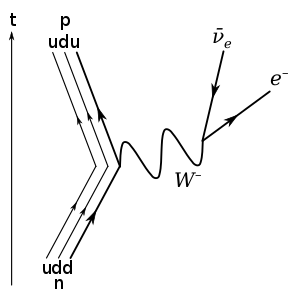
\includegraphics[width=0.65\textwidth]{Images/Theory/Beta_Decay_FD.png}
    \caption{Feynman diagram of $\beta$ decay.}
    \label{fig:BetaDecay_FD}
\end{figure}

In this interaction, the down-flavoured valence quark of a neutron (d) spontaneously decays into an up quark via the emission of a W boson. This W boson then subsequently decays into an electron and an anti-electron neutrino, leaving a traceable signature. This is known as the lepton decay mode of the W boson, and is one signature through which physicists can search for the W boson in particle collisions.

\subsubsection{The electromagnetic interaction}

The electromagnetic interaction is mediated by the photon, a spin 1 gauge boson. The conserved quantity in the SM through this interaction is hypercharge, corresponding to the U(1) gauge symmetry in the SM, illustrated in Equation \ref{eq:U1_Symmetry}. 

\begin{equation} \label{eq:U1_Symmetry}
    \phi\rightarrow\phi^{\prime}=e^{i\alpha}\phi
\end{equation}

Where $\phi$ represents a scalar field, and $\alpha$ represents a constant. Under this transformation the SM lagrangian is invariant.

The photon interacts with all electromagnetically charged particles, which includes quarks, massive leptons, and the W boson. An example interaction, that of the repulsion of two electrons via the electromagnetic force, is shown in the form of a Feynman diagram in Figure \ref{fig:EM_FD}.

\begin{figure}[H]
    \centering
    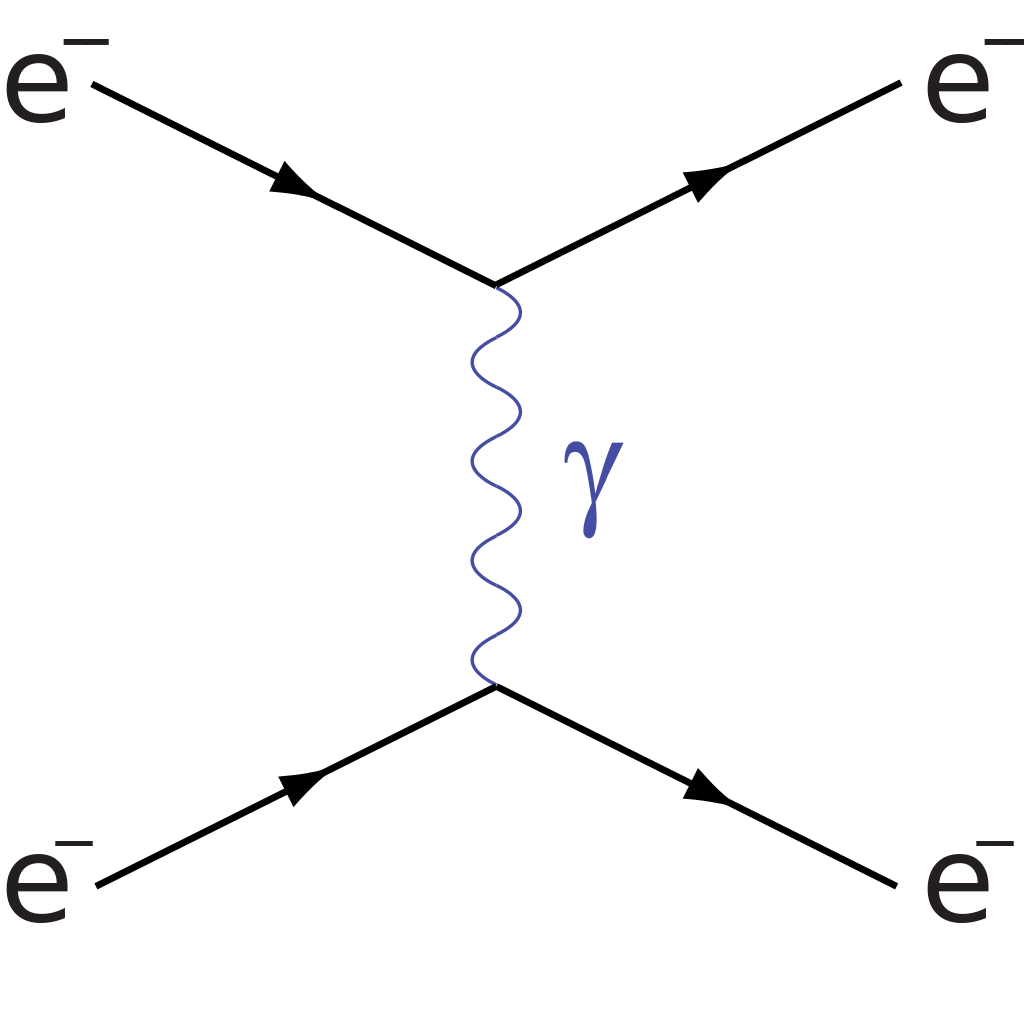
\includegraphics[width=0.65\textwidth]{Images/Theory/EM_FD.png}
    \caption{Feynman diagram of the electromagnetic interaction between two electrons.}
    \label{fig:EM_FD}
\end{figure}

\section{The higgs boson and electroweak symmetry breaking} \label{sec:Higgs}

While the electromagnetic and weak forces can be defined individually, and act separately at low energy scales, at the electroweak energy scale of about 246 GeV, they are unified into a single force called the electroweak force. This energy scale is convenient for describing the potential energy term from the Higgs boson, and the subsequent spontaneous breaking of its symmetry.

The Higgs potential term of the SM lagrangian looks as shown in Equation \ref{eqm-1}.

\begin{eqnarray}
  V(\Phi) = - \frac{\mu^2}{2}\left|\Phi \right|^2
  +\frac{\lambda}{4} \left|\Phi \right|^4
  \label{eqm-1}
\end{eqnarray}

The shape of the higgs potential is shown in Figure \ref{fig:HiggsPotential}, in a two dimensional phase space made up of the real and imaginary parts of the field $\Phi$. 

\begin{figure}[H]
    \centering
    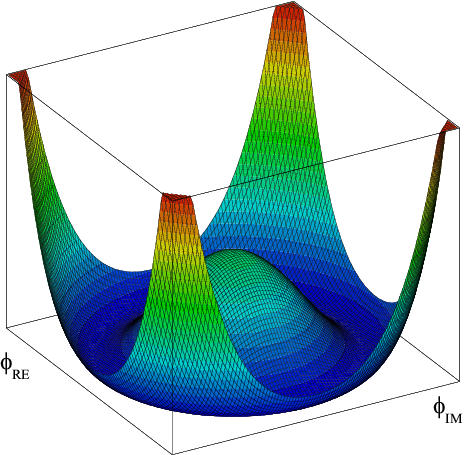
\includegraphics[width=0.65\textwidth]{Images/Theory/Higgs_Potential_Shape.png}
    \caption{Shape of the Higgs potential}
    \label{fig:HiggsPotential}
\end{figure}

A minimum energy value, or vacuum expectation value (VEV), must be taken by the higgs potential. Due to the shape of the higgs potential, an infinite number of points in the two dimensional phase space made up by the real and imaginary parts of the field $\Phi$ lie on a circle which all take on the same value of the Higgs potential. This means that a choice must be made as to which point is taken for the VEV, which leads to a spontaneous breaking of this symmetry. 

After electroweak symmetry breaking, additional terms are added to the lagrangian including mass terms for the known massive particles, and terms which determine the shape of the Higgs potential, shown in Equation \ref{eq:HiggsPotentialShape}. 

\begin{eqnarray}
  V &=& \frac{m_H^2}{2}H^2 + \lambda_3 v H^3 + \frac{\lambda_4}{4} H^4,
\quad
 \lambda_3 = \lambda_4 = \lambda_{HHH} = \frac{m_H^2}{2v^2} \label{eq:HiggsPotentialShape}
\end{eqnarray}

Thus, the shape of the higgs potential depends on the coupling strength values of a Higgs to two Higgs (the tri-linear coupling $H^{3}$), and of two Higgs to two Higgs (the quartic Higgs coupling $H^{4}$). The values of these couplings are predicted by the SM in terms of the Higgs boson mass and VEV, and based on experimental measurements the higgs self-coupling is predicted to be 0.13 by the SM.  

% After electroweak symmetry breaking, the higgs potential gains additional terms leading to the relations shown in Equation \ref{eq:Higgs_Relations}.

% \begin{eqnarray} \label{eq:Higgs_Relations}
%   \lambda = \frac{m_H^2}{2 v^2}, \;\;  \mu^2 = \frac{m_H^2}{2},
%   \;\; m_H^2 = \frac{\partial^2 V}{\partial \phi^2}
%   \label{eqm-2}
% \end{eqnarray}

% Additionally, 

Based on its predicated shape and the current measurements of the top quark mass and Higgs boson mass, the type of stability in which the Higgs VEV is predicted to sit is shown in Figure \ref{fig:HH_Stability_Plot}. 

\begin{figure}[H]
    \centering
    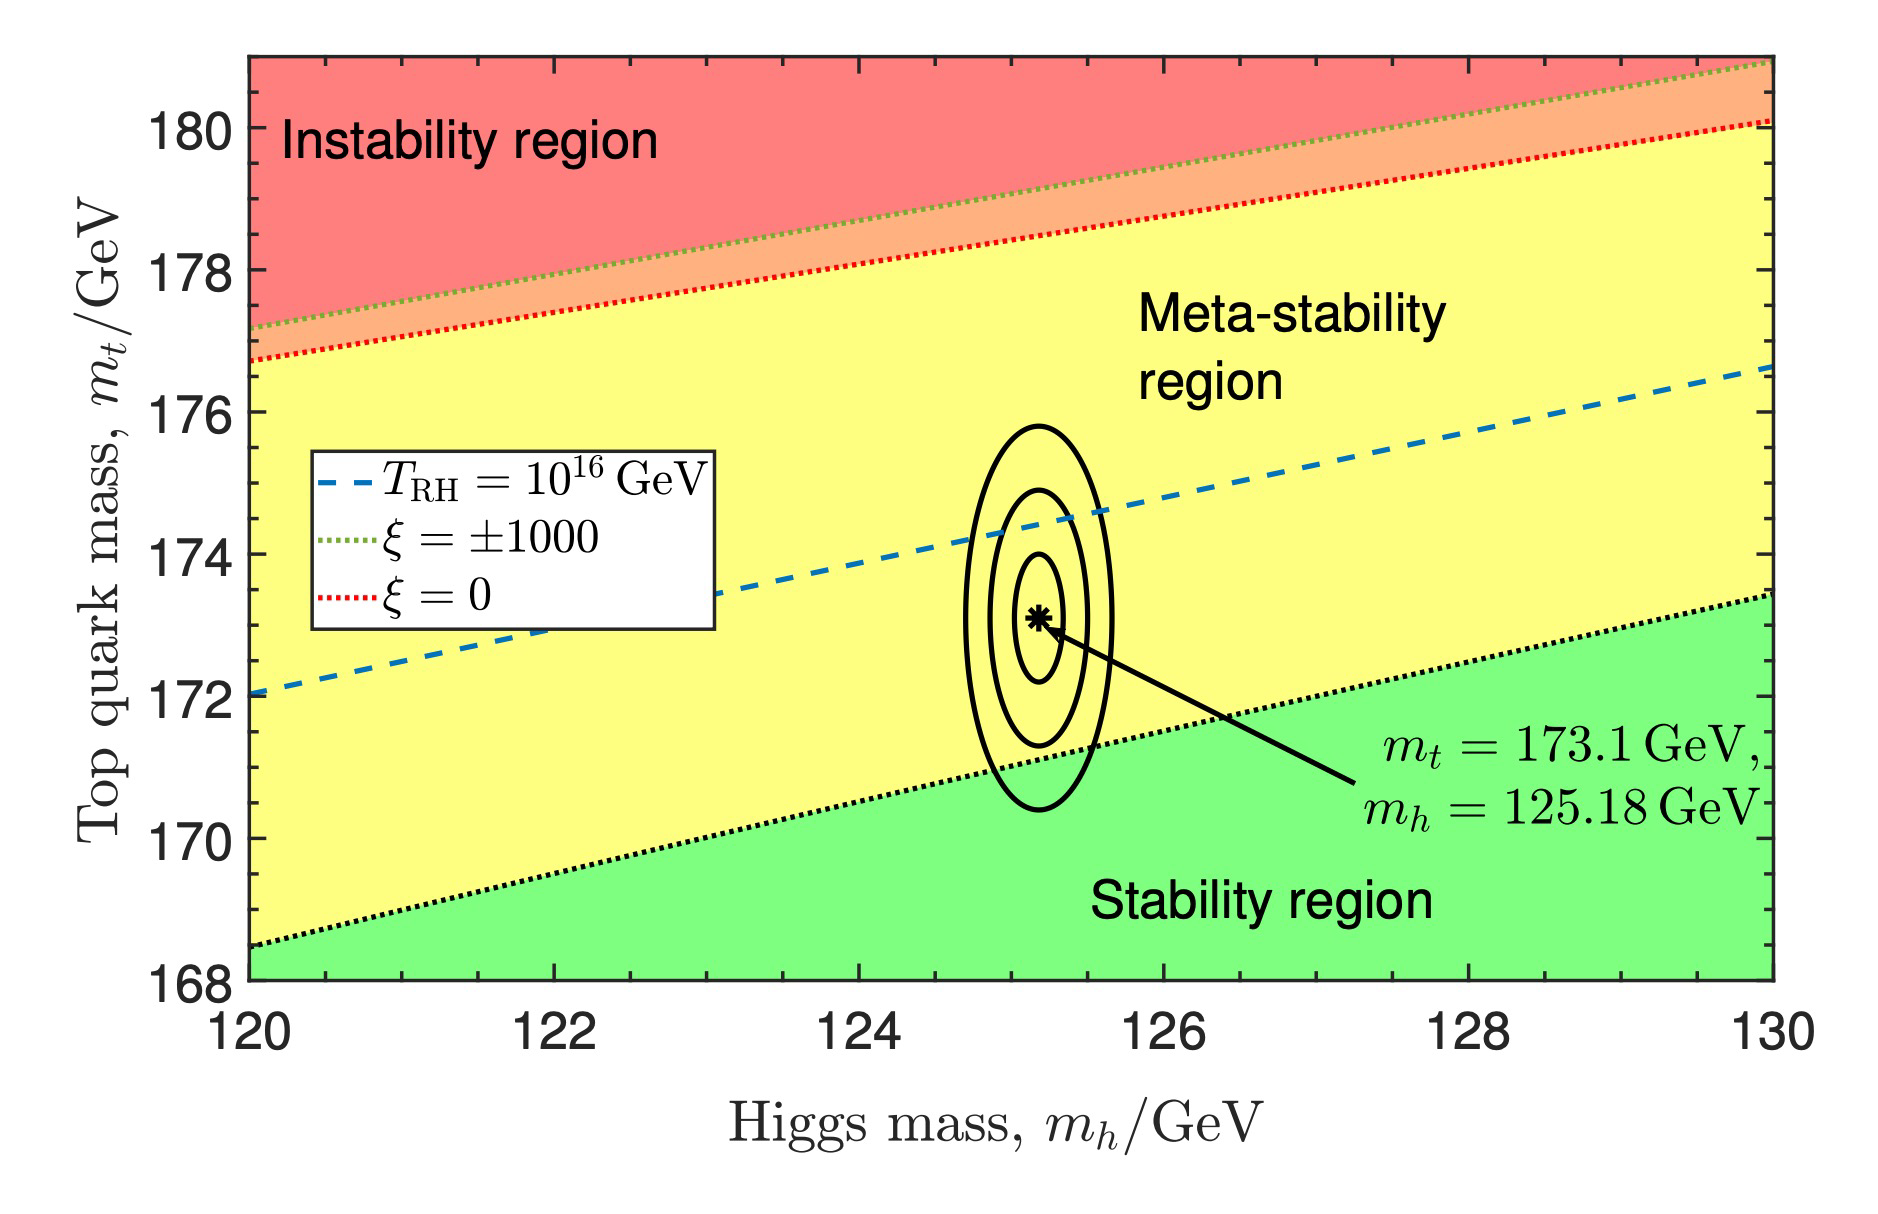
\includegraphics[width=0.65\textwidth]{Images/Theory/HH_stability_Plot.png}
    \caption{Higgs VEV stability as a function of top quark mass and Higs mass}
    \label{fig:HH_Stability_Plot}
\end{figure}

Based on current measurements of the top quark mass and Higgs boson mass, the Higgs VEV is predicted to sit at a meta-stable minimum, as depicted in Figure \ref{fig:PossibilityToTunnel}. 

\begin{figure}[H]
    \centering
    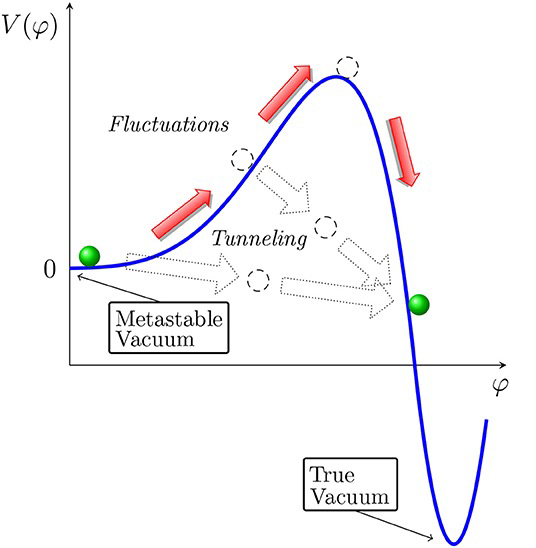
\includegraphics[width=0.65\textwidth]{Images/Theory/HH_potential_Stability.png}
    \caption{Depiction of a metastable Higgs VEV.}
    \label{fig:PossibilityToTunnel}
\end{figure}

This allows for a non-zero probability of the Higgs minimum to shift to a lower, global minimum value, through the process of quantum tunnelling. A shift of the minimum of this sort would completely change the laws of physics as we understand them. 

As this is the prediction made by the SM based on the current top quark and Higgs boson mass measurements, it is crucial to be able to compare this to experiment. This implies that an experimental measurement of the shape of the Higgs potential, accessible via its tri-linear and quartic couplings, would provide a fundamental test of the SM. 